\documentclass[12pt,oneside]{report} %12pt required by Heriot-Watt rules
\usepackage[english]{babel}
\usepackage[utf8]{inputenc}
\usepackage{csquotes} % recomended when using babel + biblatex

\usepackage[left=4cm, right=2cm, top=2cm,bottom=2cm, paper=a4paper]{geometry} %these are the HW margins
\linespread{1.5} % 1.5 line spacing required by HW

\usepackage{physics} % provides lots of nice features and commands often used in physics, it also loads some other packages (like AMSmath)
\usepackage{siunitx} % typesets numbers with units very nicely (use \SI{value}{unit commands})
\usepackage{enumerate} % allows customizing our lists
\usepackage{enumitem} % allows customizing our lists
\usepackage{amssymb} %used for \mathbb
\usepackage{amsmath} %used for \mathbb and the boxed equations
\usepackage{mathtools}
\usepackage{chemformula}%for chemical equations

%customize captions
\usepackage[labelfont=bf,textfont=it,margin=0.5in]{caption}
\usepackage{setspace} %needed for \stretch
\captionsetup{font={stretch=1}} %reduce the spacing in captions

\usepackage{graphicx} % used to place images
\usepackage{float} %provide extra options for figure placing
\usepackage[section]{placeins} %this forces figures to not leave a section
\usepackage{booktabs} %for toprule, midrule and bottomrule
\usepackage{epigraph} %used for quotes and dedication

\usepackage[toc,page]{appendix}
\usepackage{pdfpages} % to include the documents required by HW uni

\usepackage{hyperref} % for clickable references across the document
\usepackage[capitalise]{cleveref} %for references usign \cref{label}


\usepackage{dsfont} %to write the real numbers symbol
\usepackage{tikz-cd} %for fancy arrows

\usepackage[citestyle=numeric, backend=biber, sorting=none, bibencoding=utf8]{biblatex}
\addbibresource{./Bibliography.bib}

\usepackage{excludeonly} %to exclude just an include
%\excludeonly{./tex/ch6-notes} %to remove chapters
%\includeonly{./tex/titlepage2} %to include only a chapter (useful for revisions)

\renewcommand{\real}{\ensuremath{\mathds{R}}} % better real number symbol
\newcommand{\mr}[1]{\ensuremath{\mathrm{#1}}} % save some time writing equations pedices

%packages and commands for the list of publications
%these commands are for formatting the list of publications, if you decide to change formatting just change it once here.
\newcommand{\aut}[1]{#1}
\newcommand{\tit}[1]{``#1''}
\newcommand{\conf}[2]{\textit{#1}, #2}
\newcommand{\doi}[1]{\\doi:\href{http://doi.org/#1}{#1}}
\newcommand{\arxiv}[2]{\href{https://arxiv.org/abs/#1}{arXiv:#1} [#2]}
\newcommand{\jmb}{J.~MacBook}

\begin{document}

\begin{titlepage}
\newgeometry{left=2cm,right=2cm,top=1.5cm,bottom=2cm}
%this part creates the logos on top
\begin{figure}
    \centering
    \begin{minipage}{0.49\textwidth}
        \centering
        
\includegraphics[width=0.99\textwidth]{./fig/CDT-Photonics-Logo.pdf} % first figure itself
   \end{minipage}\hfill
    \begin{minipage}{0.49\textwidth}
        \centering
        
\includegraphics[width=0.5\textwidth]{./fig/HW-Logo.pdf} % second figure itself
    \end{minipage}
    % if you want a third figure, maybe your host company logo, just resize the minipages from 0.49\textwidth to 0.32\textwidth and add another minipage
\end{figure}

\title{My thesis} %these title and author and date will be saved in the pdf metadata but not displayed.
\author{Leonardo~Del~Bino}
\date{\today}

	\centering % Centre everything on the title page

	%------------------------------------------------
	%	Title
	%------------------------------------------------

	\rule{\textwidth}{1.6pt}\vspace*{-\baselineskip}\vspace*{2pt} % Thick horizontal rule
	\rule{\textwidth}{0.4pt} % Thin horizontal rule

	\vspace{0.5\baselineskip} % Whitespace above the title

	{\linespread{1.2}\scshape \huge A complicated\\
		but intriguing title\\
		spanning multiple lines\\} % Title

	\vspace{0.5\baselineskip} % Whitespace below the title

	\rule{\textwidth}{0.4pt}\vspace*{-\baselineskip}\vspace*{3.2pt} % Thin horizontal rule
	\rule{\textwidth}{1.6pt} % Thick horizontal rule

	\vspace{1\baselineskip} % Whitespace after the title block

{\LARGE John/Jane MacBook}\\%Author
\vspace{1\baselineskip}
{\large Submitted for the Degree of Doctor of Engineering\\}
\vspace{1\baselineskip}
{\scshape \large Heriot-Watt University} \\ {\scshape School of engineering and physical sciences}
 % Subtitle or further description

	\vspace*{2\baselineskip} % Whitespace under the subtitle

	%------------------------------------------------
	%	Supervisors(s)
	%------------------------------------------------

{\Large \linespread{1.2}
\begin{tabular}{ll}
	{\scshape Academic supervisor}:  & George Heriot \\
	{\scshape Industrial supervisors}: &  James Watt
\end{tabular}
}

\vfill
{\Large Month 2021\\}
\vspace*{\baselineskip}
{\footnotesize \linespread{1} The copyright in this thesis is owned by the author. Any quotation from the thesis or use of any of the information contained in it must acknowledge this thesis as the source of the quotation or information.}


\end{titlepage}
\restoregeometry
\begin{abstract}
Write your abstract here.
\end{abstract}
% This is quite simple latex code that produces a decent dedication
\begin{flushright}
    \thispagestyle{empty}
    \vspace*{\fill}
    \epigraph{To someone I care for.\\
    	Or to my cat\\
    	or some other entity.}{}
    \vspace*{\fill}
\end{flushright}
\clearpage
\chapter*{Acknowledgements}
\addcontentsline{toc}{chapter}{Acknowledgements}
One or two pages of very touchy words mixed to bad jokes where you thank your supervisors, colleagues, friends, and family for their support during the thesis writing (if they had contacts with you at the time of writing they deserve your gratitude, trust me!)
\begin{flushright}
	{\scshape John/Jane MacBook}\\
	Month 2021
\end{flushright}
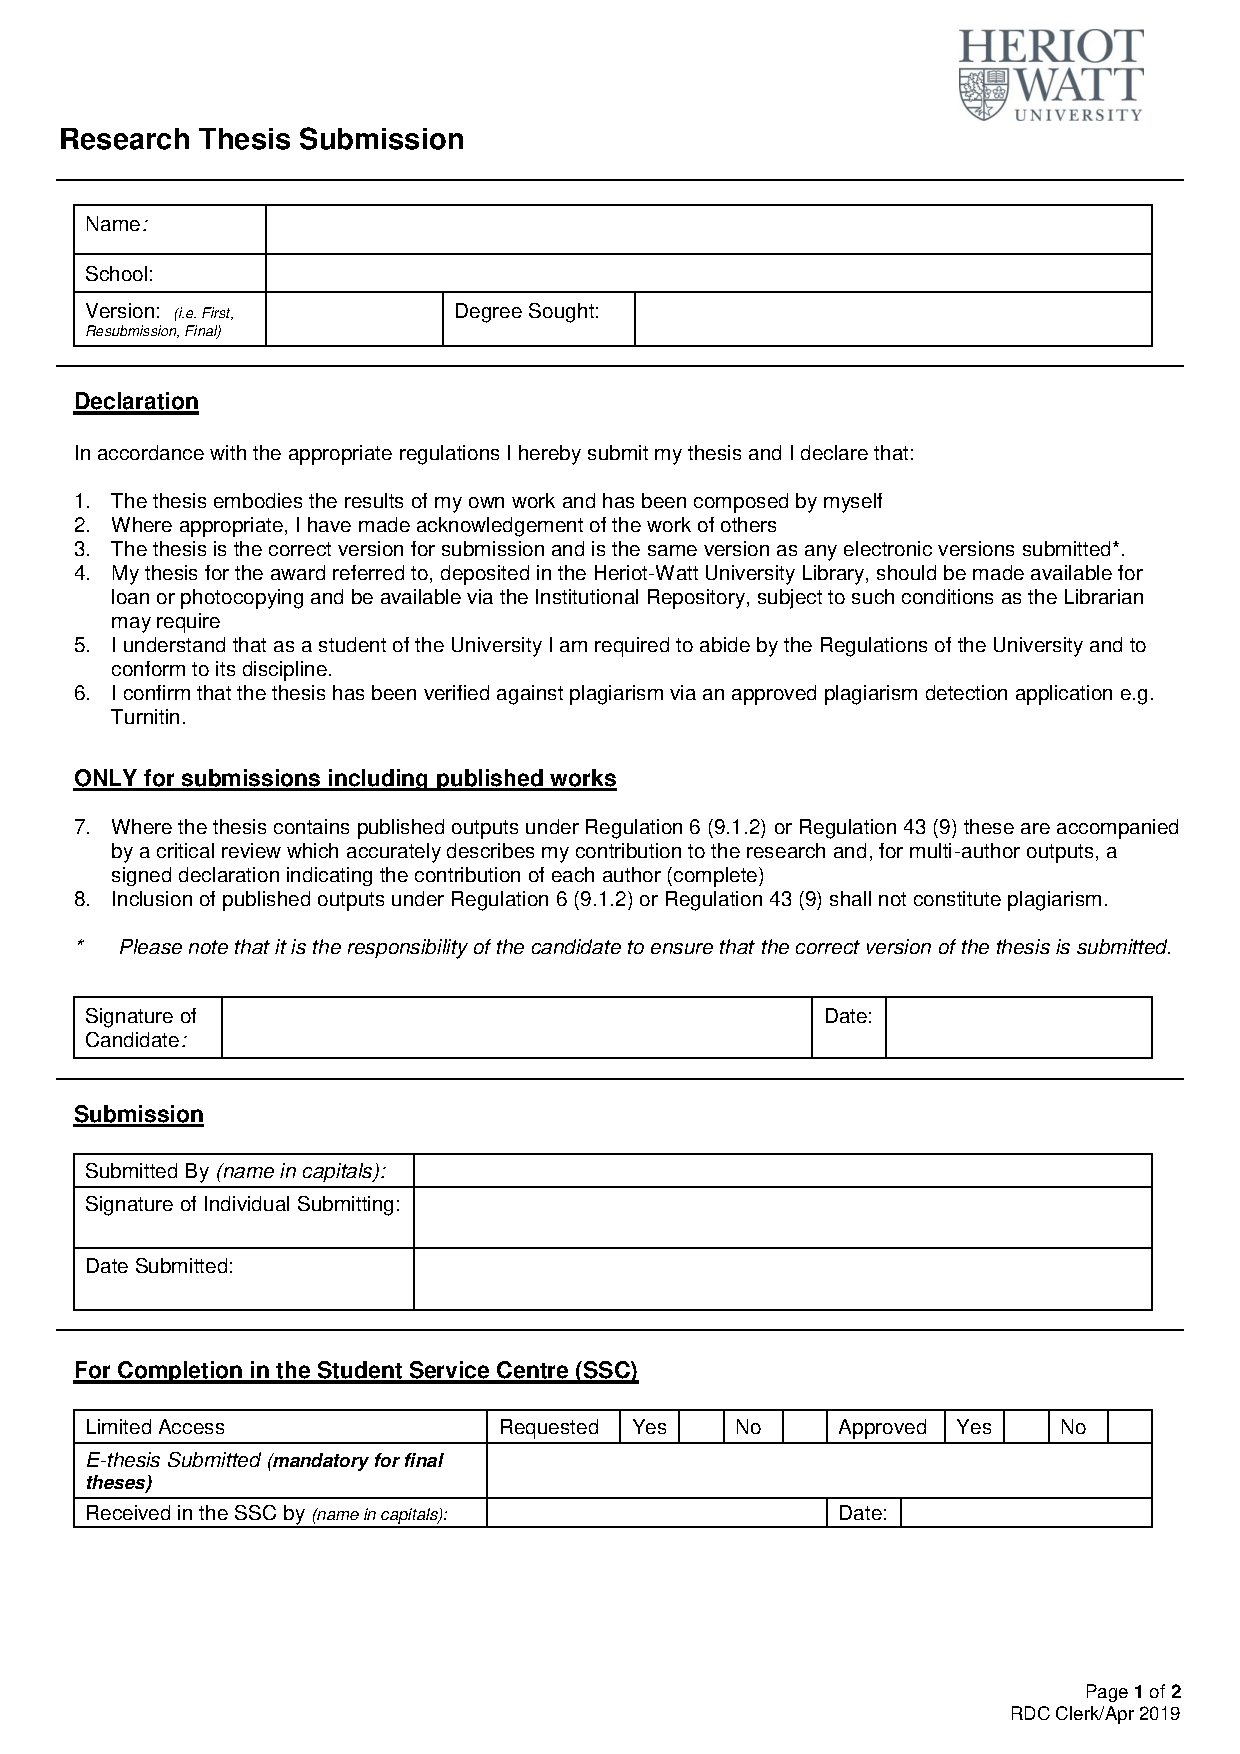
\includepdf[pages=-,pagecommand={},width=\paperwidth]{./researchthesissubmission.pdf}

\tableofcontents
\listoffigures

\chapter*{List of publications}
\section*{Publications}

\begin{description}[leftmargin=2cm, style=sameline]

	\item[Article]		\aut{J. MacBook, et al.},
	\tit{The universe and stuff},
	\textit{Nature}, vol.~1 no.~1 pp.~1-42, (15~Mar~2020)
	\doi{10.1109/JLT.2020.2975119}
\end{description}


\section*{Conferences}
\subsection*{2019}
\begin{description}[leftmargin=2.5cm, style=sameline]

	\item[Poster] 		\aut{\jmb},
	\tit{The reason why people ignore you at poster sessions},
	\conf{That conference}{Scotland 6~Nov~2019}


\end{description}
\subsection*{2018}
\begin{description}[leftmargin=2.5cm, style=sameline]

	\item[Proceeding] \aut{\jmb, et al.}
	\tit{Talking about the talk},
	\conf{CLEO}{San Jose, CA, 13-18~May~2018}
	\doi{doi.org/10.1364/CLEO\_SI.2018.SM1D.4}

\end{description}

\subsection*{Patents}
\section*{List of Symbols and notation} % Using the * doesn't make a section number
\addcontentsline{toc}{chapter}{List of Symbols and notation} % But we want the section to appear in the Table of Content

Unless specified, the lowercase letters indicate the dimensionless or normalised quantities, while the uppercase letters indicate the quantities with dimensions.

\begin{description}[leftmargin=2cm,style=sameline,noitemsep,font=\normalfont]
	\item[$P$] optical power
	\item[$I$] optical intensity
	\item[$E$] electric field
\end{description}

\begin{description}[leftmargin=2cm,style=sameline,noitemsep,font=\normalfont]
	\item[$t$] electric field transmission at the coupling point
	\item[$k$] electric field coupling at the coupling point
	\item[$\alpha$] electric field round trip transmission of the resonator
	\item[$\theta$] phase accumulated in one round trip of the resonator
	\item[$\gamma$] half width half maximum coupled linewidth
	\item[$\kappa$] coupling half linewidth
	\item[$\eta$] coupling efficiency
	\item[$\chi^{(n)}$] n-th order susceptibility
	\item[$\varepsilon_0$] vacuum permittivity
	\item[$c$] speed of light in vacuum
	\item[$L$] length of the resonator round trip
\end{description}


\section*{List of Acronyms} % Using the * doesn't make a section number
\addcontentsline{toc}{chapter}{List of Acronyms} % But we want the section to appear in the Table of Content

% Remember that the acronyms still need to be defined the first time they appear.

\begin{description}[leftmargin=2cm,style=sameline]
	\item[SPM] Self-phase modulation
	\item[XPM] Cross-phase modulation
	\item[ECDL] External-cavity diode laser
	\item[EDFA] Erbium-doped fibre amplifier
	\item[EOM] Electro-optic modulator
	\item[AOM] Acousto-optic modulator
	\item[FWHM] Full width half maximum
	\item[FSR] Free spectral range
	\item[c.c.] Complex conjugate
\end{description}
\chapter{Introduction}
\epigraph{Nothing in life is to be feared, it is only to be understood. Now is the time to understand more, so that we may fear less.}{Maria Salomea Skłodowska Curie}

A wonderful introduction to your wonderful thesis.
It may be a good idea to input separate files.
The more you divide the 200 pages document, the easier is to track what you changed and when.

\section{Literature review}
A lot of citation of the giants whose shoulders you stand \cite{Adams1979}.
\section{A section of Chapter 1}
Some text.



\chapter{Another Chapter}
\section{Code examples}
\label{sec:code_examples}

You can input equations like this if you want them on their own line:
\begin{equation}\label{eq:Q_def}
	\boxed{Q=\frac{\omega}{\Delta \omega_\mathrm{FWHM}}=\mathcal{F} \cdot \frac{\omega}{\Delta \omega_\mathrm{FSR}}}
\end{equation}

Note the \verb|\label{}| that permits to reference the equation everywhere. For example here \cref{eq:Q_def}. The equations can be inline $ Q=\frac{\omega}{2 \gamma} $.

You can include images and refer to them as shown in \cref{fig:turtle}.

\begin{figure}[ht]
	\centering
	\includegraphics[width=0.8\textwidth]{./fig/ch2/tirturtle.jpg}
	\caption{\label{fig:turtle} A picture of a sea turtle showing a wonderful animal and the effect on total internal reflection on the surface of the sea.}
\end{figure}

You can use the package chemformula to quickly input material names like this \ch{CaF2}.

It is a good idea to use the \verb|siunitx| package for the quantities since it prevents the number splitting from the unit, reduces the space between the two and can format strange units correctly. An example is \SI{0.5}{\micro m / \celsius}.
\section{Cat}
This text is from the file \verb|Thesis\tex\ch2\cat.tex|
\section{Dog}
This text is from the file \verb|Thesis\tex\ch2\dog.tex|


\appendix
\appendixpage

Write your appendix here.


\printbibliography
\end{document}